\documentclass[11pt]{article}

\usepackage{url}
\usepackage{multicol}
\usepackage[english]{babel}
\usepackage[margin=1in]{geometry}
\usepackage{graphicx}
\usepackage{subcaption}
\usepackage{enumitem}
\usepackage{amsmath}
\usepackage{amssymb}
\usepackage{wasysym}
\usepackage{color}
\usepackage{float}
\usepackage{nomencl}
\usepackage[title]{appendix}
\makenomenclature
\usepackage{pdfpages}
\usepackage{algorithm}
\usepackage{algpseudocode}
\usepackage{hyperref}
\hypersetup{
    colorlinks=true,
    linkcolor=blue,
    filecolor=magenta,      
    urlcolor=cyan,
    pdftitle={Overleaf Example},
    pdfpagemode=FullScreen,
    }
\title{16-745 Optimal Control Lecture 4}
\author{Reid Graves} 

\begin{document}
\maketitle

\section{Last Time}
\begin{itemize}
    \item Root Finding
    \item Newton's Method
    \item Minimization
    \item Regularization
\end{itemize}

\section{Today}
\begin{itemize}
    \item Line Search (fix overshooting problem)
    \item Constrained Minimization
\end{itemize}

\section{Line Search}
\begin{itemize}
    \item Often $\Delta x$ step from Newton overshoots the minimum
    \item To fix this, check $f(x + \Delta x)$ and ``backtrack" untill we get a ``good" reduction
    \item Many strategies 
    \item A simple and effective strategy is ``Armijo Rule"
    \begin{align*}
        \alpha &= 1
        \\
        \text{while } f(x+\alpha\Delta x) > f(x) + b\alpha\nabla f(x)^T\Delta x
        \\ \text{ b is tolerance, whole addition to } f(x) \text{ is expected reduction from linearization}
        \\
        \alpha \leftarrow c\alpha \text{ c is a scalar } < 1
        \\
        \text{end}
    \end{align*}
    \item Intuition
    \begin{itemize}
        \item Make sure step agrees with linearization within some tolerance $b$
    \end{itemize}
    \item Typical values:
    \begin{align*}
        c &= \frac{1}{2}, b=10^{-4} \text{ to } 0.1
    \end{align*}
    \item Take away:
    \begin{itemize}
        \item Newton with simple and cheap modifications called ``globalization strategies" is extremely effective at finding local optima
    \end{itemize}
\end{itemize}

\section{Equality constraints}
\begin{align*}
    \text{min}_x f(x) \leftarrow f(x) : \mathbb{R}^n\rightarrow \mathbb{R}
    \\
    \text{s.t. } c(x) = 0 \leftarrow c(x) : \mathbb{R}^n\rightarrow \mathbb{R}^m
\end{align*}
\begin{itemize}
    \item First-Order necessary conditions
    \begin{enumerate}
        \item Need $\nabla f(x) = 0$ in \textbf{free} directions
        \item Need $c(x) = 0$
    \end{enumerate}
    % Insert figure here
    \begin{figure}[H]
        \centering
        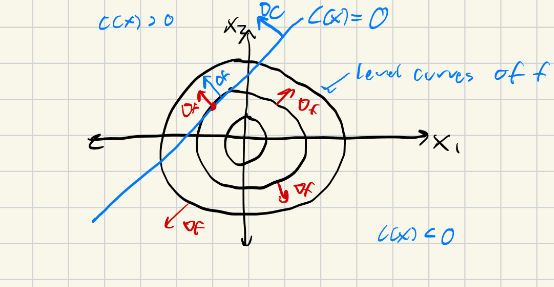
\includegraphics[width=0.7\linewidth]{lecture_4_1.png}
    \end{figure}
    \begin{align*}
        f(x) : \mathbb{R}^2 \rightarrow \mathbb{R}
        \\
        c(x) : \mathbb{R}^2 \rightarrow \mathbb{R}
    \end{align*}
    \item Any nonzero component of $\nabla f$ must be normal to the constraint at an optimum- equivalently $\nabla f$ must be parallel to $\nabla c$
    \begin{align*}
        \Rightarrow \nabla f + \lambda \nabla c &= 0 
        \\
        \lambda \text{ is Lagrange multiplier/``dual variable"}
    \end{align*}
    \item In general:
    \begin{align*}
        \frac{\partial f}{\partial x} + \lambda^T \frac{\partial c}{\partial x} &= 0, \quad \lambda\in \mathbb{R}^m
    \end{align*}
    \item Based on this gradient condition, we define:
    \begin{align*}
        L(x, \lambda) &= f(x) + \lambda^T c(x)
        \\
        \text{L is lagrangian}
    \end{align*}
    \item Such that:
    \begin{align*}
        \nabla_xL(x,\lambda) &= \nabla f + (\frac{\partial c}{\partial x}^T\lambda = 0
        \\
        \nabla_\lambda L(x,\lambda) &= C(x) = 0
    \end{align*}
    \item We can sove this with Newton:
    \begin{align*}
        \nabla_xL(x+\Delta x, + \lambda + \Delta \lambda) \approx \nabla_xL(x,\lambda) + \frac{\partial^2 L}{\partial x^2}\Delta x + \frac{\partial ^2 L}{\partial x \partial \lambda}\Delta \lambda &= 0
        \\
        \nabla_\lambda L(x+\Delta x, \lambda + \Delta \lambda) \approx c(x+ + \frac{\partial c}{\partial x} &= 0
    \end{align*}
    \begin{align*}
        \begin{bmatrix}
            \frac{\partial^2 L}{\partial x^2} & \left(\frac{\partial c}{\partial x}\right)^T \\
            \frac{\partial c}{\partial x} & 0
        \end{bmatrix}
        \begin{bmatrix}
            \Delta x
            \\
            \Delta \lambda
        \end{bmatrix}
        &= 
        \begin{bmatrix}
            -\nabla_x L(x,\lambda) \\
            -c(x)
        \end{bmatrix}
        \\
        \text{ This is ``KKT system"}
    \end{align*}
    \item Gauss-Newton Method:
    \begin{align*}
        \frac{\partial^2 L}{\partial x^2} &= \nabla^2f + \frac{\partial}{\partial x}\left[\left( \frac{\partial c}{\partial x}\right)^T \lambda  \right]
        \\
        &\text{Right additive term is expensive to compute}
    \end{align*}
    \item We often drop the 2nd ``Constraint curvature" term
    \item Called ``Gauss Newton"
    \item Slightly slower convergence than full Newton method (more iterations) but iterations are cheaper
    \item Often wins in wall-clock time
\end{itemize}

\subsection{Example}
\begin{itemize}
    \item  start $[-1,-1]$, $[-3,2]$ Full newton got stuck on $[-3,2]$, but Gauss-Newton doesn't
\end{itemize}

\begin{itemize}
    \item Take Aways:
    \begin{itemize}
        \item May still need to regularize $\frac{\partial^2 L}{\partial x^2}$ even if $\nabla^2 f>0$
        \item Gauss-Newton is often used in practice
    \end{itemize}
\end{itemize}

\section{Inequality Constraints}
\begin{align*}
    \text{min}_x f(x), \text{ s.t. } c(x)>0
\end{align*}
\begin{itemize}
    \item We'll just look at inequalities for now
    \item Just combine with previous methods to handle both kinds of constraints
\end{itemize}

\begin{itemize}
    \item First-Order Necessary Conditions:
    \begin{enumerate}
        \item $\nabla f = 0$ in the \textbf{free directions}
        \item $c(x) \geq 0$
    \end{enumerate}
    % insert figure here
    \begin{figure}[H]
        \centering
        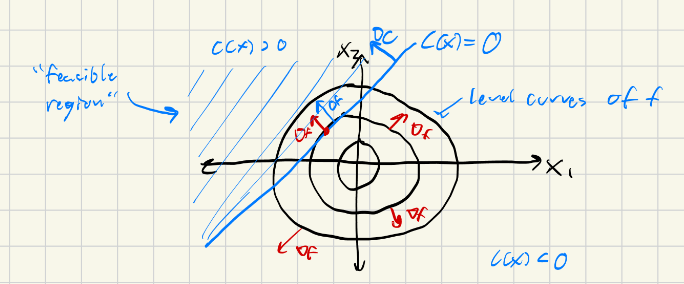
\includegraphics[width=0.7\linewidth]{lecture_4_2.png}
    \end{figure}
    \item KKT conditions:
    \begin{align*}
        \nabla f - \left(\frac{\partial c}{\partial x}\right)^T\lambda &= 0 \quad \leftarrow\text{Stationarity}
        \\
        c(x) &\geq 0 \quad \leftarrow\text{Primal feasibility}
        \\
        \lambda &\geq \quad \leftarrow\text{Dual feasibility}
        \\
        \lambda \cdot c(x) &= \lambda^T c(x) =0 \quad \leftarrow\text{Complementarity}
    \end{align*}
\end{itemize}



\end{document}
